\documentclass[a4paper,12pt,leqno]{article}
\usepackage[utf8]{inputenc}
\usepackage[T1]{fontenc}
\usepackage[polish]{babel}
\usepackage{amsmath}
\usepackage{a4wide}
\usepackage{graphicx}
\usepackage{subfig}
\usepackage{wrapfig}

\newcommand{\nel}[1]{|#1|}
\usepackage{program}

\title{\textbf{Algorytmy ewolucyjne}\\
       {\Large Raport z zadania pierwszego}\\[-1ex]}
\author{Karol Konaszyński i Wiktor Janas}
\date{Wrocław, dnia \today\ r.}

\newcommand{\avg}{\mathrm{avg}}
\newcommand{\dist}{\mathrm{dist}}
\newcommand{\median}{\mathrm{median}}
\newcommand{\target}{\mathrm{target}}
\newcommand{\RETURN}{|return|\ }

\begin{document}
\maketitle

Tematem tego projektu jest zastosowanie algorytmów ewolucyjnych do rozpoznawania obrazów. 
Problem rozpoznawania obrazów ma liczne zastosowania: od analizy zdjęć satelitarnych poprzez monitorowanie ruchu drogowego, po przemysł filmowy.
Z drugiej rozwiązanie go okazuje się być trudne, a pojęcie ,,podobieństwa obrazów'', oczywiste dla człowieka, nie jest precyzyjnie zdefiniowane.
Podejście zaproponowane w tej pracy polega na analizie samego kształtu obrazu, który uzyskujemy poprzez analizę jasności poszczególnych
pikseli (z pominięciem informacji o kolorze).

Przyjęliśmy następujące założenia: dana jest baza obrazów o zadanych nazwach (patrz rys. \ref{knownpics}). Każdy obraz, który chcemy rozpoznać
(zapytanie) jest przyrównywane dp wszystkich obrazów z bazy. Spośród obrazów bazowych wybieramy te, których odległość do zapytania jest najmniejsza.

\section{Znajdowanie punktów charakterystycznych}
Pierwszym etapem przetwarzania obrazu (pochodzącego z bazy danych lub będącego zapytaniem) jest znalezienie na nim punktów charakterystycznych.
Niech $\avg(x,y,d)$ oznacza średnią jasność obrazu w kwadracie o środku w $(x,y)$ i boku długości $d$. Dla piksela o współrzędnych $(x_0,y_0)$ oraz danej
wartości $d$ można zdefiniować funkcję
\[ F_d(\alpha) = \avg(x_0,y_0,d) - \avg( x_0+d\sin\alpha, y_0+d\cos\alpha, d) \]
Intuicyjnie jest to gradient piksela $(x_0,y_0)$ w kierunku $\alpha$ na obrazie zmniejszonym $d$-krotnie. Przyjmując kilka ustalonych wartości $d$
(w naszej implementacji były to $1,3,8$), można zdefiniować funkcję
\[ G(\alpha) = \sqrt[3]{F_1(\alpha) \cdot F_3(\alpha) \cdot F_8(\alpha)} \]
Następnie można obliczyć amplitudę tej funkcji:
\[ A = \max_\alpha G(\alpha) - \min_\alpha G(\alpha) \]
Wartość tą przyjmujemy za ,,miarę ciekawości'' piksela. 

Intuicja stojąca za tym algorytmem jest prosta -- szukamy punktów, w otoczeniu których następuje zmiana jasności obrazu. Miarą zmiany jasności w danym
kierunku jest gradient, zatem funkcja $F$ opisuje zmianę jasności obrazu we wszystkich kierunkach. Musimy jednak wziąć pod uwagę, że niektóre zmiany są
jedynie lokalne. Aby wyeleminować szum, obliczamy średnią geometryczbą funkcję $F$ dla kilku skal (jest to funkcja $G$) -- jeżeli istotnie zachodzi
rozpatrywany piksel leży w obszarze silnych zmian, nastąpi rezonans, gdy natomiast zmiana jest lokalna, funkcja większej skali ją ,,wyciszy''.
Według naszej całkowicie subiektywnej oceny skale 1,3,8 spradzają się najlepiej.

Mając określoną miarę ciekawości każdego piksela, chcemy wybrać określoną liczbę punktów charakterystycznych, które będą opisywały kształt obiektu
(liczba ta jest parametrem alogorytmu, najczęściej przyjmowaliśmy 50). Do tego celu zastosowaliśmy następujący algorytm: w każdym kolejnym kroku wybieramy
najciekawszy piksel na obrazku i dodajemy go do zbioru punktów interesujących. Nastepnie pewne jego otoczenie oznaczamy jako tabu i powtarzamy procedurę tak
długo, aż wszystkie punkty zostaną tabu. Aby określić wielkość tabu, zastosowaliśmy heurystykę ,,im ciekawiej tym gęściej''. Mianowicie, wielkość tabu jest
odwrotnie proporcjonalna do miary ciekawości punktu z pewnym współczynnikiem, który jest dobierany (za pomocą wyszukiwania binarnego) tak, aby ostateczny
zbiór punktów żądaną określoną wielkość. Proces wyszukiwania ciekawych punktów ilustruje rysunek \ref{poisrch}.

\begin{figure}\centering
\subfloat[Jabłko]{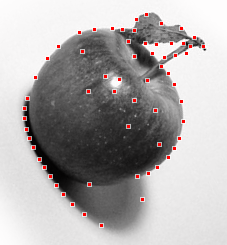
\includegraphics[width=4.5cm,keepaspectratio=true]{./apple-mod-pois.png}}
\subfloat[Wisienki]{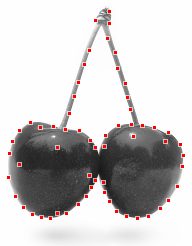
\includegraphics[width=4.5cm,keepaspectratio=true]{./cherries-pois.png}}
\subfloat[Trójliterówka]{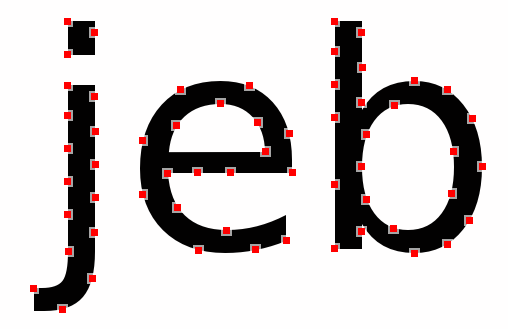
\includegraphics[width=4.5cm,keepaspectratio=true]{./jeb-pois.png}}
\caption{Przykładowe obrazy z bazy danych wraz z punktami charakterystycznymi}\label{knownpics}

\subfloat[gradient, $d = 1$]{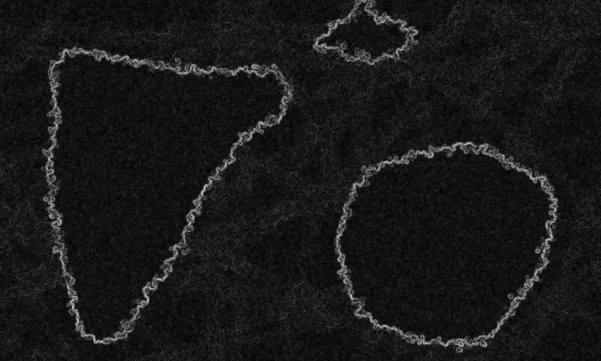
\includegraphics[width=5.75cm,keepaspectratio=true]{./noisy-grad-1.png}}\hspace{5mm}
\subfloat[gradient, $d = 3$]{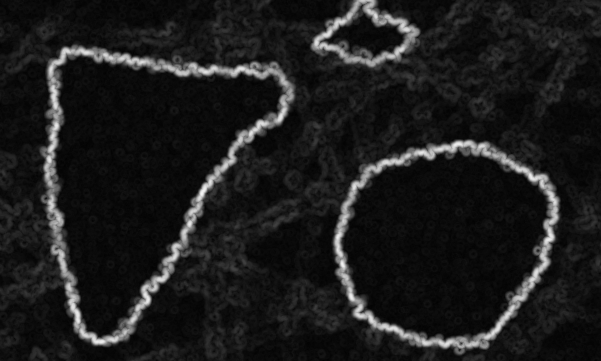
\includegraphics[width=5.75cm,keepaspectratio=true]{./noisy-grad-3.png}}\\
\subfloat[gradient, $d = 8$]{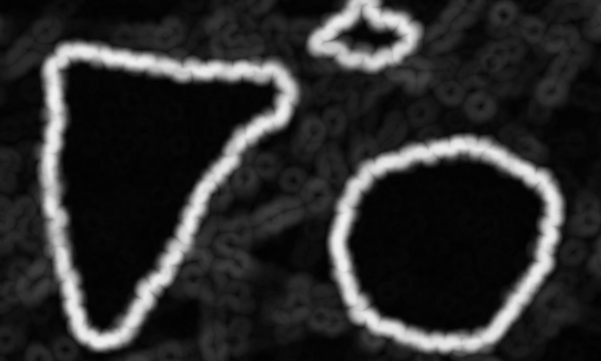
\includegraphics[width=5.75cm,keepaspectratio=true]{./noisy-grad-8.png}}\hspace{5mm}
\subfloat[gradient, łącznie]{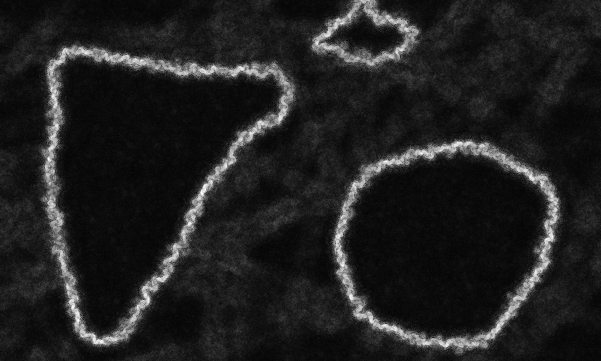
\includegraphics[width=5.75cm,keepaspectratio=true]{./noisy-grad.png}}\\
\subfloat[znalezione punkty]{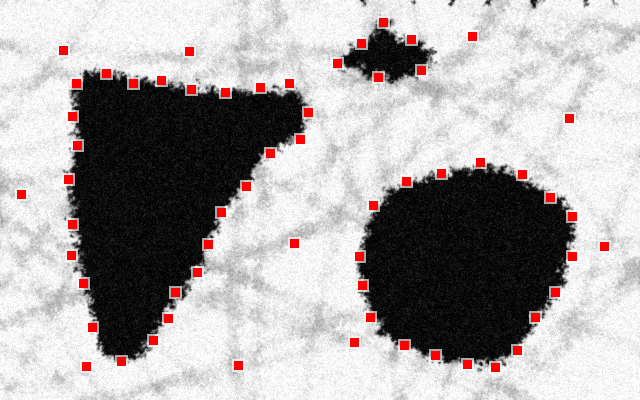
\includegraphics[width=5.75cm,keepaspectratio=true]{./noisy-pois.png}}
\caption{Proces wyszukiwania punktów charakterystycznych}\label{poisrch}
\end{figure}

\section{Analiza podobieństwa obrazów}

Mając określone punkty charakterystyczne, możemy zająć się badaniem podobienstwa obrazków.
Odległość od zbioru punktów $\bar P$ do zbioru $\bar Q$ definiujemy jako
\[ \dist(\bar P \rightarrow \bar Q) = \frac{1}{\nel{\bar P}} \cdot \sum_{p \in \bar P} \min_{q \in \bar Q}(\|p - q\|) \]
Odległość między zbiorami $\bar P$ a $\bar Q$ definiujemy jako
\[ \dist(\bar P, \bar Q) = \frac{\nel{\bar P} \cdot \dist(\bar P \rightarrow \bar Q) + \nel{\bar Q} \cdot \dist(\bar Q \rightarrow \bar P)}{\nel{\bar P} + \nel{\bar Q}} \]
Za miarę podobieństwa dwóch zbiorów punktów przyjmujemy
\[ \mathrm{similar}(\bar P, \bar Q) = \inf\{\dist(\bar P, M\bar Q) \;\arrowvert\; M\text{: afiniczne}\} \]
Jednak aby znaleźć tę musimy znaleźć przekształcenie minimalizujące wartość $\dist$. I tutaj wkracza ewolucja. 

\section{Ewolucja}

Naszymi osobnikami będą macierze afiniczne, czyli macierze postaci
$\begin{pmatrix}
\star & \star & \star \\
\star & \star & \star \\
0 & 0 & 1
\end{pmatrix}$, gdzie drugi minor główny jest złożeniem obrotu i skalowania, natomiast ostatnia kolumna odpowiada za translację.
Funkcją celu jest zatem 
\[ \target = -\dist(\bar P,  M\bar Q) \]
gdzie $\bar P$ jest wektorem punktów charakterystycznych obrazka z zapytania, zaś $\bar Q$ -- wektorem tychże dla obrazka z bazy.
Celem ewolucji jest zmaksymalizowanie funkcji celu, czyli znalezienie przekształcenia minimalizującego odległość.

Do rozwiązania tego problemu wykorzystaliśmy ideę Differential Evolution. Pseudokod zaimplementowanego algorytmu przedstawiony został na listingu: 
\begin{program}
\FUNCT |evolve| \BODY
    P := \{\}
    \FOR i := 1 \TO N \DO
        P := P + |random_translation| * |random_rotation| * |random_scaling|
    \END
    \WHILE \NOT |termination_condition| \DO
        \FOR i := 1 \TO N \DO
            |evaluate|(P_i)
        \END
        |sort|(P) 
        ~
        P := \set{P_i | i \leq N*|replace\_rate| }
        \FOR i := 1 \TO N*|replace_rate| \DO
            \IF |random|(|de_prop|)
                \THEN P := P + |de_crossover|(P);
                \ELSE P := P + |roulette_selection|(P); \FI
        \END
        ~
        \FOR i := 1 \TO N \DO 
            \IF |random|(|t_prop|)
	        \THEN P_i := |random_translation| * P_i; \FI
            \IF |random|(|s_prop|)
                \THEN P_i := |random_scaling| * P_i; \FI
            \IF |random|(|r_prop|)
                \THEN P_i := |random_rotation| * P_i; \FI
	    \IF |random|(|f_prop|)
                \THEN P_i := |random_flip| * P_i; \FI
        \END
    \END
\END
~
\FUNCT |de_crossover|(P) \BODY
    x1 := |roulette_selection|(P)
    x2 := |roulette_selection|(P),\; x1 \neq x2
    x3 := |roulette_selection|(P),\; x3 \neq x1,\; x3 \geq x2
    \RETURN x1 + (x3-x2) * f_\text{de}
\END
~
\FUNCT |termination_condition| \BODY
    \RETURN |gen_idx| > G \OR 
	    |max_target|(|gen_idx|, |gen_idx|-K) \geq |max_target|(|gen_idx|-K, |gen_idx|-2*K)
\END
\end{program}

Najpierw odbywa się losowa inicjacja populacji z parametrem N. Następnie wchodzimy w pętlę ewolucji, która wykonuje się aż nie zostanie spełniony
warunek zakończenia. W pętli, pierwszą czynnością jest ewaluacja każdego osobnika, czyli znalezienie dla niego wartości target oraz fitness,
gdzie fitness jest współczynnikiem przystosowania:
\[ \mathrm{fitness}(p) = \frac{\target(p) - \min_{q \in P}\target(q)}{\sum_{r \in P} \target(r) - \min_{q \in P}\target(q)} \]
Wartość fitness jest wykorzystywana do uporządkowania osobników od najlepszego do najgorszego oraz podczas selekcji ruletkowej.
Potem następuje selekcja blokowa połączona z krzyżowaniem, ostatecznie zaś mutacja każdego osobnika. Warunkiem zakończenia ewolucji
jest przekroczenie pewnej ustalonej ilości pokoleń (zwykle rzędu 200) bądź stwierdzenie, że w czasie ostatnich $K$ pokoleń nie nastąpiła
poprawa w stosunku do poprzednich $K$ pokoleń ($K$ jest również parametrem).

Krzyżowanie polega na wybraniu metodą ruletki trzech różnych osobników $x_1, x_2, x_3$ a następnie utworzeniu z nich osobnika postaci
$x1 + f_\text{de}\cdot(x3-x2)$, gdzie $f_\text{de}$ jest parametrem, zaś operacja dodawania i mnożenia jest zwykłą operacją dodawania
macierzy i mnożenia ich przez skalar.

Ważną obserwacją którą poczyniliśmy jest to, że nie warto dokonywać losowych skalowań, czy obrotów wokół punktu $(0,0)$, gdyż to spowoduje duże
zmiany w położeniu punktów oddalonych od środka układu współrzędnych (czyli lewego górnego rogu). Aby tego uniknąć, obroty i skalowania wykonujemy
względem punktu wybranego z małego otoczenia punktu $(\median(\bar X), \median(\bar Y))$, gdzie $\bar X, \bar Y$ są zbiorami współrzędnych x, y
punktów charakterystycznych.

\subsection{Parametry algorytmu}

Działanie algorytmu jest uzależnione od wielu parametrów. Wszystkie one zostały wyodrębnione z kodu programu. Ich wartości są następujące:

\begin{tabular}{l|l|l}
parametr                & wartość & znaczenie \\
\hline
\texttt{threads}        & 2     & ilość wątków obliczeniowych\\
\hline
\texttt{poiSteps}       & 16    & skok funkcji gradientu od kąta \\
\texttt{poiScales}      & 1,3,8 & skale gradientów \\
\texttt{poiCount}       & 60    & ilość punktów charakterystycznych (POI) \\
\texttt{poiThreshold}   & 30    & próg poniżej którego nie uznajemy punktu za POI \\
\hline
\texttt{populationSize} & 400   & wielkość populacji \\
\texttt{survivalRate}   & .8    & współczynnik przetrwania \\
\texttt{stopCondParam}  & 40    & wartość K używana w warunku zakończenia \\
\texttt{maxGeneration}  & 200   & maksymalna ilość pokoleń \\
\hline
\texttt{translateInit}  & 0.5   & początkowy rozrzut translacji\\
\texttt{rotateInit}     & 6.283 & początkowy rozrzut rotacji\\
\texttt{scaleInit}      & 4     & początkowy rozrzut skali \\
\hline
\texttt{translateProp}  & .03   & prawdop. translacji podczas mutacji \\
\texttt{rotateProp}     & .03   & prawdop. obrotu podczas mutacji \\
\texttt{scaleProp}      & .03   & prawdop. skalowania podczas mutacji \\
\texttt{flipProp}       & .05   & prawdop. odbicia względem prostej podczas mutacji \\
\hline
\texttt{translateDev}   & .5    & odchylenie w losowaniu translacji (w mutacji) \\
\texttt{rotateDev}      & .05   & odchylenie w losowaniu obrotu (w mutacji) \\
\texttt{scaleDev}       & .05   & odchylenie w losowaniu skalowania (w mutacji) \\
\texttt{originDev}      & 0.3   & rozrzut przy wyborze punktu srodka obrotu i skali \\
\hline
\texttt{deMatingProp}   & 0.8   & prawdop. krzyżowania \\
\texttt{deMatingCoeff}  & 0.1   & współczynnik w krzyżowaniu \\
\texttt{deMatingDev}    & 0.05  & rozrzut powyższego \\
\end{tabular}

\section{Eksperymenty}

Przeprowadzane eksperymenty podzielono na kilka grup: rozpoznawanie owoców, cyfr, słów trzyliterowych oraz obrazków bardzo zaszumionych.
Pojedyńczy eksperyment polega na ustaleniu grupy obrazków bazowych (rzędu 10 - 20), wybraniu obrazka do zapytania, który jest podobny do
któregoś z bazowych a następnie uruchomieniu algorytmu i wypisaniu pięciu najbardziej podobnych obrazków bazowych wraz z ich odległościami.
Na tej podstawie staramy się okreslić, czy program rzeczywiście udzielił poprawnych odpowiedzi. Przedstawimy tutaj zarówno eksperymenty udane
jak i nieudane, aby wyciągnąć kilka wniosków na przyszłość.

\subsection{Szukanie jabłka wśród owoców}
Prosty, ale ważny test, który dobrze ilustruje działanie programu. Baza owoców zawiera zdjęcia pojedynczej wiśni, podwójnych wisienek, banana, 
jabłka, ananasa, porcji arbuza, papryki i gruszku. Zapytaniem jest identyczne jak w bazie jabłko, poddane jedynie obrotowi i przesunięciu.
Oczekiwanym przez nas wynikiem jest zwrócenie przez algorytm listy najbardziej podobnych owoców z jabłkiem na szczycie listy i odległością jak
najbliższą zera. Technicznie rzecz biorąc istnieje przekształcenie afiniczne, które perfekcyjnie przekształca jabłko z bazy danych na jabłko z
zapytania. Jednak algorytm nie porównuje bezpośrednio obrazków, a jedynie ich punkty charakterystyczne. Ponieważ algorytm wyszukiwania punktów
charakterystycznych daje nieco inne odpowiedzi dla jabłka z bazy i jabłka z zapytania, znalezienie dopasowania o odległości zero jest niemożliwe.

Na wykresie \ref{applemod} przedstawione są wartości funkcje celu najlepszych osobników w kolejnych pokoleniach. Ze względu na zrandomizowany
charakter algorytmu, to samo zapytanie wykonano dziesięć razy i uśredniono wyniki (to znaczy: przedstawiony wykres dla \texttt{banana} jest w
istocie średnią z dziesięciu uruchomień dla \texttt{banana}; analogicznie z pozostałymi obrazkami). Okazuje się, że ostateczna odległość
obrazka z zapytania od jabłka z bazy jest niewielka, istotnie mniejsza niż pozostałych owoców. Eksperyment uznajemy za udany, zgodnie z oczekiwaniami.

\begin{figure}\centering
\footnotesize\include{applemod-vs-fruits}\vspace{-2em}
\normalsize\caption{Dopasowanie owoców (\texttt{fruits}) do obróconego jabłka (\texttt{applemod}); uśrednione wyniki z dziesięciu uruchomień programu.}\label{applemod}
\end{figure} 

\subsection{Dopasowanie wisienek}
Dość trudny test. Zapytanie to podwójne wisienki, bardzo podobne do podwójnych wisienek z bazy, jednak posiadające dodatkowo listek na ogonku. 
Obecność listka znacznie zaburza rozkład punktów charakterystycznych, jednak, co powoduje, że podobieństwo obrazków jest nietrywialne. 
Oczekiwanym wynikiem jest jednak wciąż najlepsze dopasowanie dla wisienek. Oto wynik działania algorytmu:
\begin{verbatim}
cherries, fruits (-12.547963)
banana, fruits (-14.550430)
pineapple, fruits (-14.859610)
paprika, fruits (-14.931395)
watermelon, fruits (-15.112849)
\end{verbatim}
Udało się! Zgodnie z oczekiwaniami, zwycięzca nie jest tak wyraźny jak było to w przypadku jabłka, jednak cel został osiągnięty. Znalezione dopasowanie
przedstawione jest na rysunku \ref{cherries}. Czerwonymi kropkami zaznaczono punkty charakterystyczne wisienek z bazy danych (bez listka), zaś 
niebieskimi punktami -- wisienek z zapytania (z listkiem).

\subsection{Inne eksperymenty z owocami}

\paragraph{Gruszka}
W tym eksperymencie będziemy porównywać zdjęcie gruszki do bazy owoców. Oczywiście, oczekujemy, że najbliższym owocem okaże się także gruszka.
Ten eksperyment jest prosty, gdyż gruszki są do siebie podobne. Wynikin, jak widać, są zgodne z oczekiwaniami. Co więcej, całkiem dobrze do
gruszki dopasowała się papryka. Dopasowania te przedstawiają rysunki \ref{pear} oraz \ref{paprika}.
\begin{verbatim}
pear, fruits (-16.697315)
paprika, fruits (-18.802341)
banana, fruits (-19.460381)
cherry, fruits (-21.882196)
watermelon, fruits (-23.120878)
\end{verbatim}

\paragraph{Ananas}
Bardzo ciekawym eksperymentem okazało się wyszukiwanie ananasa. Kształt ananasa jest bardzo charakterystyczny i powoduje powstanie bardzo
dobrze rozłożonych punktów charakterystycznych, szczególnie w obszarze korony. Jednak kształt ten jest też bardzo nieregularny, i choć
,,na oko'' ananasy są do siebie podobne, punkty charakterystyczne dwóch różnych zdjęć mogą się bardzo istotnie różnić. Z drugiej strony,
w bazie danych nie znajduje się żaden owoc choć trochę podobny do ananasa (nie będący ananasem), zatem są nadzieje, że eksperyment powiedzie
się. Otrzymane wyniki pokazują, że istotnie najlepsze dopasowanie otrzymano dla ananasa, jednak odległość do kolejnego obrazu (melona) jest
bardzo niewielka. Co więcej, program dopasował ananasy... do góry nogami! Dopasowanie to przedstawiono na rysunku \ref{pineapple}.
\begin{verbatim}
pineapple, fruits (-11.685663)
watermelon, fruits (-12.371205)
apple, fruits (-12.665856)
paprika, fruits (-13.042226)
pear, fruits (-13.062563)
\end{verbatim}

\begin{figure}\centering
\subfloat[\texttt{cherries} do \texttt{cherries6}]{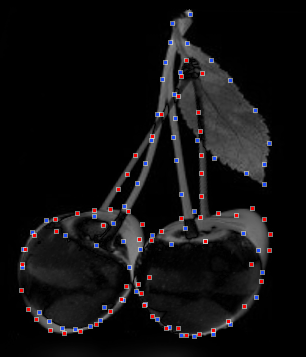
\includegraphics[width=7.5cm,keepaspectratio=true]{./cherries-match.png}\label{cherries}}\hspace{5mm}
\subfloat[\texttt{pineapple} do \texttt{pineapple3}]{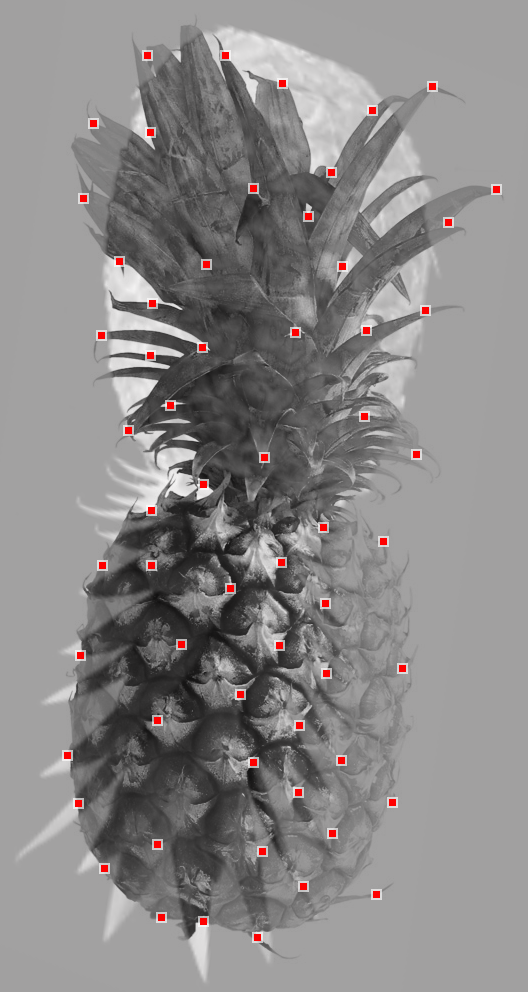
\includegraphics[width=7.5cm,keepaspectratio=true]{./diff_pineapple.png}\label{pineapple}} \\
\subfloat[\texttt{pear} do \texttt{pear2}]{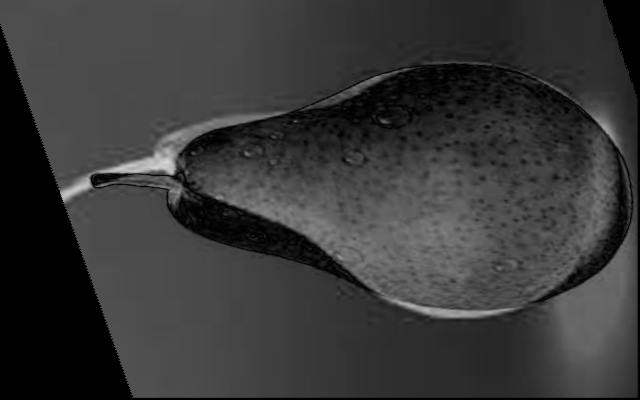
\includegraphics[width=7.5cm,keepaspectratio=true]{./diff_pear.png}\label{pear}}\hspace{5mm}
\subfloat[\texttt{paprika} do \texttt{pear2}]{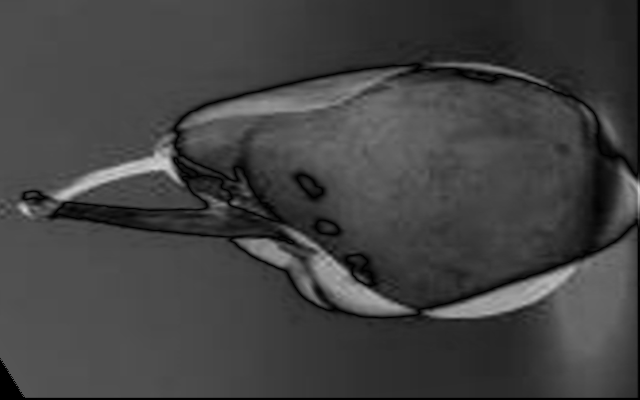
\includegraphics[width=7.5cm,keepaspectratio=true]{./diff_paprika.png}\label{paprika}}
\caption{Przykładowe dopasowania owoców}\label{matches}
\end{figure}

\subsection{Rozpoznawanie trójliterówek}
Kolejną grupą eksperymentów, którymi zajmiemy się w tym raporcie, będzie próba dopasowania tych samych słów (trzyliterowych) ale napisanych inną czcionką.
Wbrew pozorom, nie jest to zadanie łatwe - na rozkład POI w bardzo dużym stopniu zależy od grubości linii w czcionce kąta nachylenia pisma. Okazuje się jednak, że większość nieskomplikowanych 
testów nasz program przechodzi poprawnie.
Baza słów wygląda następująco: car cut bra sex six jeb map rap two bar sut. Napisane są czcionką Sans.
\paragraph{Słowo cut}
W tym teście spróbujemy rozszyfrować słowo cut napisane inną czcionką. Jest bardziej pochyła i ma cieńszą linię.
Wyniki jednak cieszą:
\begin{verbatim}
cut, 3letters (-10.864353)
sut, 3letters (-11.867450)
car, 3letters (-12.411745)
bra, 3letters (-13.751248)
rap, 3letters (-14.585580)
\end{verbatim}
Dopasowanie słowa cut napisanych różnymi czcionkami przestawione jest na rysunku \ref{cut}.
Zgodna z oczekiwaniami jest także niewielka odległość słów cut i sut - w końcu mają dwie litery wspólne.

\paragraph{Słowo jeb}
Ten test jest dobrym przykładem tak zwanego Pyrrusowego zwycięstwa. Zapytaniem jest słowo jeb, obrócone o 90 stopni napisane pochyłą czcionką.
Nasz algorytm znajduje poprawne dopasowanie -- \ref{jeb} -- ale wyższą wartość ma słowo sex -- \ref{jeb_sex}.
Jednak wyniki są znowu zaskakujące:
\begin{verbatim}
sex, 3letters (-10.982061)
two, 3letters (-11.131102)
jeb, 3letters (-11.574780)
sut, 3letters (-11.622553)
cut, 3letters (-11.646334)
\end{verbatim}
Udało nam się wychwycić słabą stronę algorytmu; kształt jest inny, jednak przypadkowo dopasował się wyjątkowo dobrze. Niestety, trudno takich błędów się pozbyć. W tym teście nie uzyskaliśmy 
optymalnego wyniku, jednak dwa cele zostały osiągnięte -- oczekiwane słowo znajduje się w pierwszej trójce propozycji oraz znaleźliśmy poprawne dopasowanie między tymi samymi słowami.








\subsection{Rozpoznawanie obrazów zaszumionych}
tutaj napisać, ze w wyniku zniekształcenia obrazka zaszumionego (noisy vs. noisy-mod) zmieniają się bardzo-bardzo poi i że algorytm nie znajduje nic mądrego

\subsection{Rozpoznawanie geometrii}
tutaj działające square vs. romb oraz niedziałające stripes / dots


\section{Wpływ wartości parametrów algorytmu na wyniki}

\begin{figure}\centering
\subfloat[Ananas i Ananas]{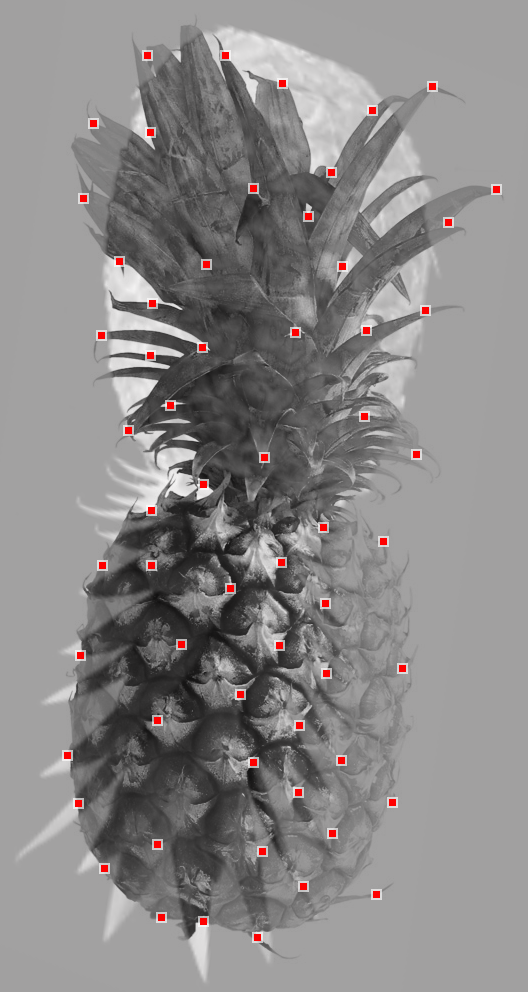
\includegraphics[width=6cm,keepaspectratio=true]{./diff_pineapple.png}}
\subfloat[POI ananasa]{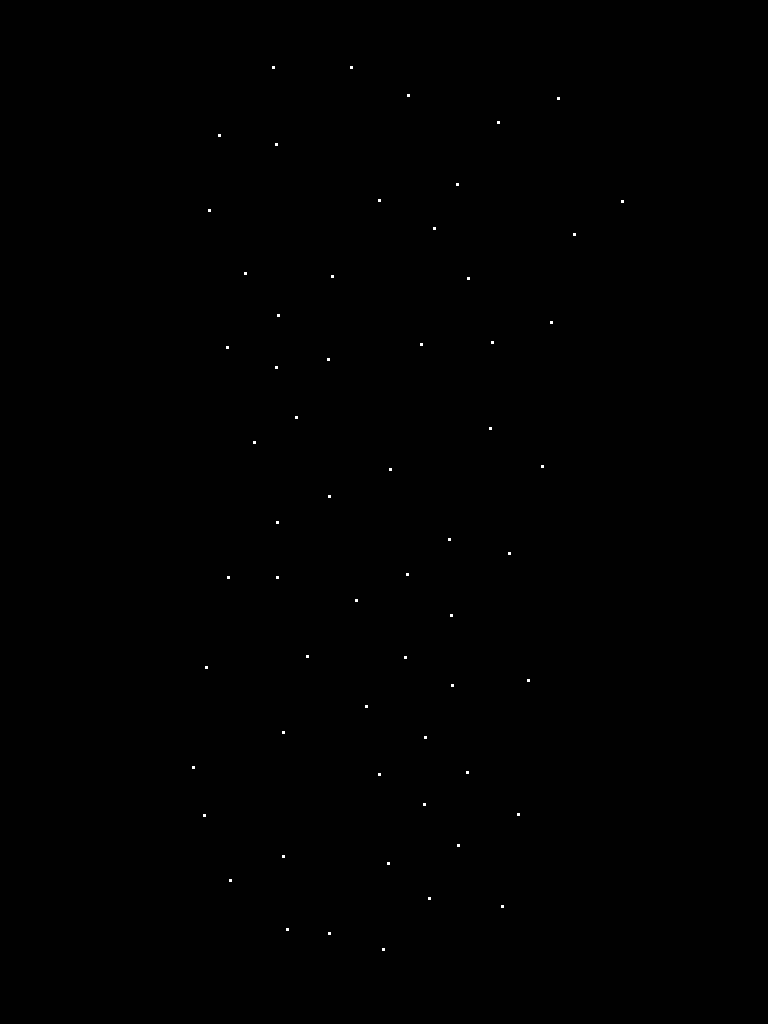
\includegraphics[width=6cm,keepaspectratio=true]{./pineapple_pois.png}}
\caption{Dopasowanie \texttt{pineapple} do \texttt{pineapple3} oraz punkty charakterystyczne tego drugiego}
\end{figure}

\begin{figure}\centering
\subfloat[\texttt{cut} do \texttt{cut}, różne czcionki]{
\includegraphics[width=6cm,keepaspectratio=true]{./diff_cut_cut.png}\label{cut}}\hspace{5mm}
\subfloat[\texttt{jeb} do \texttt{jeb}, różne czcionki]{
\includegraphics[width=6cm,keepaspectratio=true]{./diff_jeb_jeb.png}\label{jeb}}
\subfloat[\texttt{sex} do \texttt{jeb}]{
\includegraphics[width=6cm,keepaspectratio=true]{./diff_jeb_sex.png}\label{jeb_sex}}
\caption{Dopasowania niektórych słów trzyliterowych}
\end{figure}




\begin{figure}\centering
\footnotesize\include{square-vs-romb-popsize}\vspace{-2em}
\normalsize\caption{Wpływ rozmiaru populacji na ewolucję (dopasowanie \texttt{square} do \texttt{romb}); uśrednione wyniki z dziesięciu uruchomień programu.}
\end{figure}
\begin{figure}\centering
\footnotesize\include{square-vs-romb-deprop}\vspace{-2em}
\normalsize\caption{Wpływ prawdopodobieństwa krzyżowania na ewolucję (dopasowanie \texttt{square} do \texttt{romb}); uśrednione wyniki dziesięciu uruchomień programu.}
\end{figure}
\begin{figure}\centering
\footnotesize\include{square-vs-romb-surv}\vspace{-2em}
\normalsize\caption{Wpływ współczynnika przetrwania na ewolucję (dopasowanie \texttt{square} do \texttt{romb}); uśrednione wyniki dziesięciu uruchomień programu.}
\end{figure}

\section{Uwagi implementacyjne}

Program wymaga systemu operacyjnego GNU/Linux. Do jego kompilacji niezbędne są, poza standardowymi narzędziami, pliki nagłówkowe biblioteki GTK+,
zazwyczaj dostępne w pakiecie \texttt{libgtk2.0-dev} lub podobnym. Aby skompilować program należy w katalogu ze źródłami wydać polecenie \texttt{make}.
W wyniku jego wykonania powinien powstać plik wykonywalny o nazwie \texttt{evolution}. Program przyjmuje dwa parametry, plik z obrazkiem-zapytaniem oraz
nazwę grupy obrazków z bazy danych. Przykładowe wywołanie może zatem wyglądać następująco:
\begin{verbatim}./evolution fruits/apple-mod.pgm fruits\end{verbatim}
Powyższe polecenie powoduje porównanie obrazka \texttt{fruits/apple-mod.pgm} do wszystkich obrazków z kategorii \texttt{fruits}.
Kategorie są opisane w pliku \texttt{evolution.database} i można je edytować. Gdy program otrzymuje obraz do analizy po raz pierwszy, niezbędne jest
wyszukanie punktów charakterystycznych. Jest to długotrwała czynność (może trwać nawet pół minuty dla jednego obrazka), jednak znalezione punkty
charakterystyczne są zapisywane na dysk i przy kolejnych uruchomieniach program będzie korzystał z obliczonych wcześniej danych. Program wczytuje
obrazy w formacie \texttt{pgm}, wraz z kodem źródłowym dostarczane są przykładowe obrazy (w katalogach \texttt{digs}, \texttt{fruits}, \texttt{geom},
\texttt{noise} oraz \texttt{text}). Uwaga: program nie potrafi wczytać obrazów, które zawierają komentarze. Pliki \texttt{pgm} tworzone przez program
GIMP zawierają komentarz (i nie jest nam znana żadna metoda skłonienia GIMPa do nie umieszczania komentarza w plikach \texttt{pgm}). Wraz z kodem
źródłowym dostarczono skrypt \texttt{rmhash}, który usuwa komentarze z plików \texttt{pgm}.

Kod źródłowy podzielony jest na kilka plików. Główna część programu znajduje się w pliku \texttt{evolution.C}. Plik \texttt{poi.C} zawiera algorytm
wyszukiwania punktów charakterystycznych. Plik i \texttt{image.C} oraz \texttt{composite.C} zawierają kod operacji na obrazkach. Pliki \texttt{gui.C}
oraz \texttt{gui-gtk.c} zawierają implementację graficznego interfejsu użytkownika. Plik \texttt{workers.C} zawiera framework dla przetwarzania
wielowątkowego, zaś plik \texttt{config.C} zawiera parser konfiguracji.

\end{document}
